\textit{Dette kapitel omhandler alle systemets blokke og herigennem deres design, implementering og test. Hver enkelt blok vil først blive behandlet for sig selv, hvorefter de vil blive behandlet som et samlet system. Alle blokke er designet ud fra deres kravspecifikationer og testes ligeledes herudfra. Afslutningsvis vil kapitlet omhandle en test af det samlede system med henblik på dets funktionelle krav og kravspecifikationer.}

Systemet er opbygget af forskellige blokke, der designes, implementeres og testes separat. Afslutningsvis koples hver blok sammen, som til sidst testes som et samplet system. De enkelte blokke af systemt designes med henblik på at sikre systemets funktionalitet, hvorfor de designes med henhold til de opstillede krav i \secref{Sec:krav}. Systemet vil dermed overordnet have en opbygning, som illustreres på \figref{fig:design_blokdiagram}.
\begin{figure}[H]
	\centering
	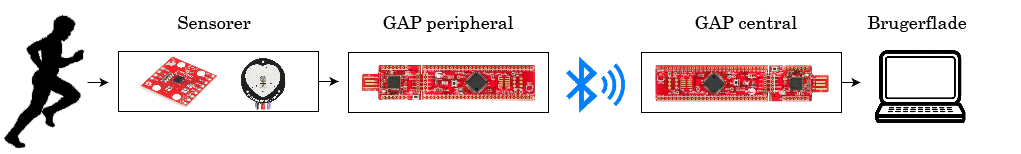
\includegraphics[scale=0.45]{figures/bProblemloesning/blokdiagram.png}
	\caption{På figuren ses blokdiagrammet for det samlede system illustreret med de benyttede komponenter. Inputsignalet modtages fra sensorer påført en bruger, hvorefter en databehandling i GAP peripheral detekterer, hvilken type aktivitet der udføres. Efterfølgende benyttes BLE til dataoverførsel fra GAP peripheral til GAP central. Afslutningsvis er der en brugerflade visualiseret på en computer.}
	\label{fig:design_blokdiagram}
\end{figure}
Blokkene implementeres forskellige steder i det samlede system, som vist på \figref{fig:design_blokdiagram}. Spændingsforsyningen tilkobles GAP peripheral MCUen, hvor sensorer også tilkobles. På denne MCU vil signalerne blive digitaliseret og algoritmer vil efterfølgende behandle og adskille aktiviteterne gang, løb og cykling samt udregne en tilhørende puls. Algoritmen og krav hertil står i \secref{krav_algoritme} som én samlet enhed, men i det efterfølgende vil der være to algoritme afsnit: en til behandling af data fra henholdsvis accelerometer og gyroskop. Disse data sendes via BLE til en GAP central, som er koblet til en computer. På computeren vil dataet blive visualiseret igennem en MATLAB GUI, hvor brugeren kan følge sin progression.